%---------------------------------%
% Article Body
%---------------------------------%
\documentclass[../article.tex, 12pt]{subfiles}
\begin{document}

%---------------------------------%
% Title
%---------------------------------%
\begin{center}
{\bfseries\Huge Identifying Cannabis Dispensary Purchase Patterns with Market Basket Analysis}
\end{center}

\vspace*{-1\baselineskip}
\begin{center}
{\Large By Paul Kitko}
\end{center}

%---------------------------------%
% Abstract
%---------------------------------%
\pdfbookmark[1]{Abstract}{Abstract}
\Abstract{\hspace{4ex}Market Basket Analysis (MBA) sometimes referred to as Association Rule Mining, Affinity Analysis or Frequent Itemset Mining, was developed as a method to evaluate ``if / then'' associations that arise between elements in a dataset \citep{agrawal1994fast}. Historically MBA rule sets have been applied to retail grocery stores' Point of Sale data to develop likely product associations that can then be used to anticipate and recommend combinations of future purchases. These recommendations or ``cross-sells'' have been found to be useful in improving retail sales volume. The newly legalized recreational cannabis market offers an opportunity to apply MBA to an unexplored retail industry. This project used MBA on a retail cannabis dataset representing multiple dispensaries across the state of Washington. The project's purpose was to verify if MBA was feasible in uncovering useful product association rules from a cannabis sales dataset to use in cross-selling recommendations. The results of the study show that it is possible to derive meaning MBA rule sets from cannabis retail data but that some limitations were uncovered that offer three future opportunities for research. First that similar product with highly differentiated names may need to be re-categorized into more generalized and meaningful products. Second, that it is possible that product churn may introduce signal noise into the MBA process resulting in a higher number of less useful rule sets. Third, that cannabis customers tend to purchase within product families which is an atypical finding in MBA and should be further explored.
}
\vspace*{-1\baselineskip}
\begin{center}
{\sffamily Dispensary Comparison by Levels of Median Household Income}\vspace*{0.25\baselineskip}\\
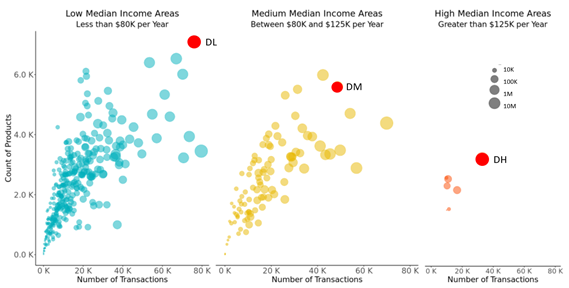
\includegraphics[width=0.8\linewidth]{figures/figure-5.png}
\end{center}
\vspace*{0.125\baselineskip}

%---------------------------------%
% Material
%---------------------------------%
\begin{multicols*}{2}
\pdfbookmark[1]{Introduction}{Introduction}
\section{Introduction}
\label{sec:introduction}

\thispagestyle{titlepage}

Market Basket Analysis (MBA) sometimes referred to as Association Rule Mining, Affinity Analysis or Frequent Itemset Mining, was developed as a method to evaluate ``if / then'' associations that arise between elements in a dataset \citep{agrawal1994fast}. For example, in American grocery store transactions, if customers buy a product like peanut butter, then MBA can show how likely those customers are to buy the other complimentary products to make a sandwich, like bread and jelly. The associations that emerge from MBA can be grouped together to form ``rules'' that are useful in understanding consumer purchasing patterns. Historically MBA association rules add evidence-based insights that inform retail marketing strategies. Applied MBA has led to improved cross-selling opportunities, creation of attractive product bundling promotions \citep{malati2017}, generated customer friendly retail floorplans \citep{hipp2000algorithms} and has even been used to develop improved item pairings for restaurant menus \citep{ting2010finding}. Uncovering associations with MBA has proven so versatile that it has also been applied to diverse fields like genomics, aviation, energy, and medical diagnosis, but a review of literature shows that most of MBA's contributions are made in the retail space. 

\par
An area of unprecedented retail growth where advanced analytical techniques like MBA have seen very little use is in the US recreational cannabis market. According to analysis by \citep{flowhub2021}, a cannabis data and software platform company, the US cannabis market is expected to be worth between \$80 and \$100 billion by 2030. To date 17 states have legalized the use of recreational cannabis driving growth and clearing the way for establishing retail outlets, called dispensaries. Each state also recognizes cannabis as a controlled substance, and as such, it must be managed and regulated across the entire supply chain. This concept is commonly known as ``seed to sale'' (STS) tracking \citep{kees2020evidence}. As the name implies, STS tracking starts with sourcing seeds or plant clones. From there, planting, cultivation and, harvesting activities are tracked by producers buy tagging ``batches'' of product commonly referred to as flower or bud, with barcoded Radio Frequency ID tags. While harvesting, batch samples are transported via certified delivery companies to cannabis testing labs for contaminant compliance. The same delivery companies also ship tested batches to processors who turn the raw cannabis flower into derived products like edibles, inhalers, and oils. These derived products are also tracked with barcoded RF ID tags. All products, whether in raw form direct from the producer or derived products from a processor, are shipped to dispensaries for final sale to the customer.

\par
Each state's cannabis market requires a STS platform that collects and tracks each transaction for compliance and tax purposes. These platforms are developed by third party vendors and generate an immense amount of data at each stage of the STS value chain. The final link in the chain is the dispensary, and when equipped with point-of-sale data tracking systems integrated with the STS platform, opens the door to many of the same data-driven marketing opportunities that conventional retailers use like MBA.

\pagestyle{regular}

\pdfbookmark[2]{Inspiration}{Inspiration}
\subsection{Inspiration}

The inspiration for this project comes from two sources. The first is the opportunity to apply proven data science concepts to a new data source from a relatively untapped market, thereby increasing the chances of making a concrete contribution. The second is to assist a new software services startup company called Cannlytics based in Olympia, Washington. Cannlytics is owned by Keegan Skeate and currently specializes in developing productivity improvement software for cannabis testing labs. Conducting retail sales analysis in the form of MBA explores a part of the STS value chain that Cannlytics can offer as a new service to potential customers.

\pdfbookmark[2]{Objectives and Purpose}{Objectives and Purpose}
\subsection{Objectives and Purpose}

The project's overall objective is to show if MBA can uncover retail purchasing patterns (association rules) in a large STS cannabis data set and if those patterns can be leveraged by dispensaries to make cross-sell marketing decisions. The project's results will serve as either a potential service that the client can offer to retail dispensaries or as content for a whitepaper that the client can use as promotional research material.

\par
This project will explore association rules generated from specific product names generated from the sales of three representative dispensaries and results will be contrasted to make recommendations on how to use the data. Sub-objectives to achieving the main goal include:
\begin{itemize}
\item	Explain, in accessible terms appropriate for the client, what MBA is, how it works and how it is useful in retails sales.

\item	Procure a representative STS cannabis data set containing raw retail sales transactions appropriate for conducting MBA. This project will be using a dataset supplied by the Washington State Liquor and Cannabis Board.

\item	Due to the size of the Washington State STS database, this project will leverage a cloud computing environment for data preprocessing, querying and MBA model development. 

\item	Use exploratory data analysis to understand the data sets and identify a group of representative dispensaries that make suitable candidates for a comparative MBA analysis.

\item	Develop key visual results that Cannlytics can leverage as a possible sales tool for offering MBA services to dispensaries.

\end{itemize}

\pdfbookmark[2]{Limitations}{Limitations}
\subsection{Limitations}

Due the substantial size of STS datasets, considerations must be made to effectively handle the data. Effectively uploading, preprocessing, and querying the raw data must be taken into account. I selected Google Cloud's Big Query service for these activities due to its ease of use when compared to alternatives like Amazon Web Services and Microsoft Azure. Big Query leverages standard SQL for data manipulation. Developing the MBA model will also be accomplished in Google Cloud using their AI Platform. Derived modeling datasets are anticipated to be quite large (sparse matrices) but the AI Platform environment should have ample computing resources to process it. All AI Platform MBA models will be developed in the R programming language within a ``notebooks'' environment.

\pdfbookmark[2]{Organization of the Paper}{Organization of the Paper}
\subsection{Organization of the Paper}

The paper's structure is as follows:

% TODO: Create links to subsections.
{\hypersetup{linkcolor = black}
\begin{enumerate}

\item \hyperref[sec:introduction]{Introduction}

\begin{enumerate}
\item Overview of market basket analysis and its applicability to cannabis retail;
\item Inspiration;
\item Objectives and purpose;
\item Limitations.
\end{enumerate}

\item \hyperref[sec:literature-review]{Review of Current Literature and Research}

\begin{enumerate}
\item Origins and development of MBA;
\item Understanding MBA association rules and measuring their strength;
\item Use cases for MBA;
\item Recent developments in MBA research.
\end{enumerate}

\item \hyperref[sec:methodology]{Methods}

\begin{enumerate}
\item Data acquisition and understanding seed-to sale data schema;
\item Transformation of data formats, perform data quality checks;
\item Exploratory data analysis to identify candidate retail dispensaries;
\item MBA data preprocessing and modeling.
\end{enumerate}

\item \hyperref[sec:results-and-discussion]{Results}

\begin{enumerate}
\item Fine-tuning MBA association rules;
\item Applicability of results for retail dispensaries.

\end{enumerate}

\item \hyperref[sec:conclusion]{Conclusion}

\begin{enumerate}
\item Summary and takeaways;
\item Recommendations for further development.
\end{enumerate}

\end{enumerate}
}

\pdfbookmark[1]{Literature Review}{Literature Review}
\section{Literature Review}
\label{sec:literature-review}

The introduction of legalized recreational cannabis in 17 states has dramatically increased the number of retail dispensaries across the country. Like any traditional retail outlet, dispensaries are faced with typical marketing decisions to increase product sales. Typical retail practices are being used but to date there is very little evidence to suggest that sophisticated analytical technique like MBA have been employed in the cannabis industry. This literature review confirms that dispensaries have made little progress using advanced analysis to support traditional retail decisions at the consumer level. More specially, this review highlights the potential for using MBA to develop cross-selling strategies in the emerging cannabis market.

\pdfbookmark[2]{The Link Between Market Basket Analysis and Cross-selling}{The Link Between Market Basket Analysis and Cross-selling}
\subsection{The Link Between Market Basket Analysis and Cross-selling}

Many traditional retail sales strategies have been refined using MBA to increase customer sales. Cross-selling, up-selling, store layout optimization, product shelf placement, customer affiliation marketing and product bundling have all been used based on MBA-generated association rules \citep{kamakura2008cross, derdenger2013dynamic, ting2010finding, bermudez2016layout, berg2018emerging}. Cross-selling appears to be the most popular retails sales strategy in much of the MBA literature and is intended to increase customer ``share of wallet'' while providing value-added goods and services. According to \cite{kamakura2008cross} there are five advantages to cross-selling:
\begin{enumerate}
\item It takes much less time to cross-sell a new product to an existing customer that trying to recruit a new customer to the same product.
\item Cross-selling response rate are between 2 to 5 times more effective than cold-calls.
\item There is evidence that suggests cross-selling deepens the customer to seller relationship improving prospects for increased ``share of wallet.''
\item Deeper customer relationships lead to improved customer retention.
\item The customer to seller relationship deepens as the seller learns more about the customers wants and needs resulting in a competitive advantage.
\end{enumerate}

The five advantages of traditional cross-selling create an obvious business incentive, but it wasn't until retail technology developments in the early 1990's that cross-selling could be scaled and adopted across the retail industry.

\pdfbookmark[2]{Market Basket Analysis and Cross-selling Adoption in Retail}{Market Basket Analysis and Cross-selling Adoption in Retail}
\subsection{Market Basket Analysis and Cross-selling Adoption in Retail}

The adoption of MBA for cross-selling can be attributed to the proliferation of PoS (Point of Sale) systems. Traditionally salespeople would broker cross-sell opportunities, but PoS systems have turned human-mediated sales into streamlined transactions that collect and store vast amounts of consumer data \citep{kamakura2008cross}. Advancements in data storage drove down the cost of storing PoS data and improved processing capability which made analyzing very large data sets feasible \citep{avcilar2014association}. By early 1990's the convergence of affordable storage and improved processing power with ubiquitous PoS systems opened the door to a variety of data analysis techniques including MBA. Combining MBA with cross-selling became an obvious approach once PoS technology was in place.

\par
The concept behind cross-selling is that a retailer can offer customers alternate products and services based what they have already purchased. Said another way, cross-selling poses the question, ``If you like this, then you may like that.'' The cross-selling idea aligns nicely with the ``if/then'' MBA association rules, mentioned previously, that arise between elements in a dataset \citep{agrawal1994fast}. The conceptual overlap between MBA and cross-selling has led to a variety of applications to the retail market.

\pdfbookmark[2]{Market Basket Analysis and Cross-selling Use Cases}{Market Basket Analysis and Cross-selling Use Cases}
\subsection{Market Basket Analysis and Cross-selling Use Cases}

Foundational work from Agrawal, Imielinski and Swami introduced MBA in 1993 and it quickly became one of the most used algorithms in retail. MBA refers to the act of multiple shoppers loading various products into their respective shopping baskets resulting in interesting aggregate combinations. These combinations can then be analyzed to potentially improve product offerings \citep{avcilar2014association}. A survey of the literature reveals a diverse set of MBA use cases.

\par
In one interesting example, MBA was used to develop an ``ideal'' menu assortment of entrees and side dishes for a restaurant \citep{ting2010finding}. The authors examined over 3,700 dining transactions for the associations generated between 24 entrees and 49 side dishes. The combinations uncovered with the highest frequency and strength of association were then used to make dining suggestions to undecided customers. The cross-sell suggestions generated in the study were welcomed by customers two out of three times.

\par
In a separate study, MBA was applied to improving grocery store layouts, commonly called block designs \citep{ozgormus2020data}. The underlying logic goes like this: MBA was used to identify those product combinations of most interest to the customers. The combinations were optimized in conjunction with the store' physical layout and those product combinations that could realize the most cross-sell revenue. From there a set of block designs were created from which the retailer could choose the most appropriate one.

\par
MBA not only offers a data driven approach to block designs, but optimized floorplans can also be used to improve cross-sell promotional strategies in the store. \cite{bermudez2016layout} first analyzed 24 product families for association rule strength. The resulting associations were then positioned in the store in such a way as to maximize the travel distance customers take to collect complementary products. The strategy of maximizing travel distance means customers are exposed to additional offerings during their shopping visit which raises the likelihood of unplanned purchases. Once the block design was implemented promotional advertisements were placed adjacent to complimentary products incentivizing trips though the store to gather the additional cross-sell goods.

\par
These examples show MBA can play a key role in data driven retail strategies like cross-selling, but this versatile data mining technique has been applied to many domains other than retail. Genetics research by \cite{anandhavalli2010association} developed association rules that determine the relationships between a single gene expression and thousands of other genes expression patterns. In another interesting use case, \cite{bhagwandin2017association} generated association rules with MBA to show which home appliances are used in conjunctions with others to determine energy saving patterns. These patterns, when used by smart home management systems as a rule set, were able to automatically turn on and off co-used appliances to increase energy efficiency. A recent study by \cite{natalia2020apriori} used association rule mining to uncover which conditions were most associated with aircraft runway excursions (accidents) at airports. In this study the equivalent of the retail transactions that we see in traditional MBA are the taxi routes aircraft takes before or after takeoff. Various contributing factors like type of aircraft, aircraft systems fault and human error were then used to generate patterns associated with the runway excursion incidents. 

\pdfbookmark[2]{Criticisms and Considerations}{Criticisms and Considerations}
\subsection{Criticisms and Considerations}

For all its support and broad application MBA does have some detractors. \cite{zhang2021measuring} argue that although MBA uncovers associations rules it falls short in attributing any linkage to consumer demographics. Zhang argues that rules may have weak associations in aggregate but when attributed to consumer subpopulations the strength of association can be substantially increased. Essentially Zhang sees this as a lost opportunity to better inform retail decision making. An additional criticism from \cite{vindevogel2005promotion} goes a step further suggesting that complimentary elements of associations rules (the products) can be substituted thereby making the association rules useless to retailers. Instead Vindevogel suggested promoting sales based on cross-price elasticities.

\par
Cross-selling does have its limitations and may not be appropriate in all circumstances. For cross-selling to work it must be seen by the customer as a beneficial service and not just a sales tactic. For instance, not meeting the customers original needs first before introducing cross-selling suggestions or ``over-touching'' can result in turning off the customer \citep{kamakura2008cross}. Additionally, if a cross-selling strategy is employed on the sales floor, then salespersons should exercise the skills for making recommendations to customers based on MBA analysis and results. Salespeople must also be effectively incentivized to deliver appropriate cross-selling suggestions to customers. A balance must be met to not overly incentivize salespersons leading to disruptive competition at the expense of the customers' experience \citep{kamakura2007chain}. Although these criticisms and limitations may have merit in their specific use cases this project defers to the broad and proven application of MBA to cross-selling.

\pdfbookmark[2]{How does Market Basket Analysis Work?}{How does Market Basket Analysis Work?}
\subsection{How does Market Basket Analysis Work?}

At its core, MBA is an exploratory data mining technique used to derive frequent and highly associated ``in/then'' patterns from large retail datasets. Foundational work from Agrawal, Imielinski and Swami introduced MBA in 1993 and it became one of the most popular algorithms in retail. MBA refers to the act of multiple shoppers loading various products into their respective shopping baskets resulting in interesting aggregate combinations. These combinations can then be analyzed to potentially improve product offerings \citep{avcilar2014association}.

\par
As previously mentioned, MBA and the association rules it generates are derived from PoS transactional datasets, but two challenges arise when generating association rules from large data sets. The first is that the number of rule combinations grow exponentially with the size of the database. It's easy to imagine the huge number of rule combinations that can be generated from a grocery store filled with thousands of products. The second challenge is selecting interesting subset of rules form a potentially large pool \citep{hipp2000algorithms}. The first challenge is addressed with a concept called the apriori principal which ``prunes'' the size of association rule sets and the second challenge is managed by applying thresholds called support, confidence, and lift that restrict the size and applicability of the association rules. Let's look at the first challenge in more detail.

\par
The apriori principal asserts that if an item set (association rule) is infrequent then all supersets that contain the same item set must also be infrequent. For example, in a grocery store, if cookie sales are infrequent then cookie and milk sales should also be infrequent. The concept is quite intuitive and regulates association rule frequencies. The name apriori originates from idea that association rules use ``prior knowledge'' about subsets to deduce what can be contained in a superset. The apriori principal was incorporated into the ``apriori algorithm'' developed by \cite{agrawal1993mining} in their landmark paper, ``Mining Association Rules between Sets of Items in Large Databases.'' The paper established the foundational concepts for MBA. As a testament to this paper's importance to the data mining community, as of this writing Google Scholar showed over 23,000 citations.

\par
As mentioned previously, there is second method to limiting a potentially large number of MBA association rules. The second method is based on the understanding that association rules generated by the apriori algorithm come in the form of two ``if/then'' parts. The first part is called the antecedent and the second part is called the consequent. The rule format takes the form of {antecedent} $\Rightarrow$ {consequent} which is read as ``antecedent implies consequent.'' Here are some examples:
\begin{equation*}
\{\text{peanut butter}\} \Rightarrow \{\text{jelly}\}
\end{equation*}
\begin{equation*}
\{\text{hotdogs}\} \Rightarrow \{\text{buns}\}
\end{equation*}
\begin{equation*}
\{\text{hotdogs, buns}\} \Rightarrow \{\text{ketchup}\}
\end{equation*}
\begin{equation*}
\{\text{hotdogs, buns}\} \Rightarrow \{\text{ketchup, mustard}\}
\end{equation*}

Notice the hotdog examples. Both the antecedent and consequent can have more than one item. Intuitively it's easy to understand how quickly the number of combinations can grow from large retail data sets. Due to the power of the apriori algorithm it's possible to limit the number of association rules generated by incorporating thresholds called support, confidence, and lift.

\par
Support is a measure of how frequent an association rule is in proportion to the total number rules generated from a dataset. Support can be thought of as measure of a rule's ``popularity.'' For example, if the rule \{hotdogs, buns\} $\Rightarrow$ \{ketchup\} occurs 10 times in set of 100 possible association rules the support value is 10/100 or 0.1:
\begin{equation*}
\text{Support} = \frac{\{\text{hotdogs, buns}\} \Rightarrow \{\text{ketchup}\}}{\text{Total}}
\end{equation*}

What's convenient when using the apriori algorithm is that you can set a support threshold to discriminate infrequently occurring rule sets. In the example above if we set support to .2 then the \{hotdogs, buns\} $\Rightarrow$ \{ketchup\} rule would not be included in the result set of association rules helping surface more frequently occurring rules. Support can never have a value greater than 1 due to the apriori principal.

\par
Another threshold used for association rules is called confidence. Confidence is the implied strength between the antecedent and the consequent and can be thought of as how likely the consequent would occur given the antecedent was purchased:
\begin{equation*}
\text{Confidence} = \frac{\{\text{hotdogs, buns}\} \Rightarrow \{\text{ketchup}\}}{\{\text{hotdogs, buns}\}}
\end{equation*}

Like support, confidence can be set to a minimum value thus discriminating lower value associations that are not deemed as important for making retail decisions. Confidence values are also limited to value less than or equal to 1, but some caution should be considered when using it. In the above formula the antecedent's popularity is taken into account but the consequent's popularity is not. If the consequent is also popular then there is a possibility that confidence could be artificially inflated. To address the possibility of artificial inflation the measure of lift is used. Lift works the same way confidence does except it controls for how popular the consequent is:
\begin{equation*}
\text{Lift} = \ddfrac{\frac{\{\text{hotdogs, buns}\} \Rightarrow \{\text{ketchup}\}}{\{\text{hotdogs, buns}\}}}{\frac{\{\text{ketchup}\}}{\text{Total}}}
\end{equation*}

Lift values greater than 1 show strength of association with larger values indicating more strength. For this project lift will be the primary measure used to evaluate MBA associations rules in the Washington State retail cannabis dataset.

\pdfbookmark[2]{An Opportunity to Apply Market Basket Analysis to Cannabis Dispensaries}{An Opportunity to Apply Market Basket Analysis to Cannabis Dispensaries}
\subsection{An Opportunity to Apply Market Basket Analysis to Cannabis Dispensaries}

To date the literature shows very little research in cannabis retail sales analysis other than high-level parallels to the cannabis market drawn from the tobacco and alcohol industries \citep{berg2018emerging}. Results from Berg's Marijuana Retail Surveillance Tool survey confirmed that dispensaries are employing several strategies to improve product availability, price, and promotion. Price discounts, social media promotions, loyalty programs and indoor signage for novel products were being used to influence customer buying decisions but Burg made no mention of more sophisticated marketing techniques being used. Additional research for this project identified a single vendor called Headset which claims to offer ``basket analysis'' for its clients but a deeper investigation into the offering revealed that the firm offers summary statistics of items purchased at an aggregate market basket level and not true MBA association rules that are applicable to cross-selling strategies. The lack of evidence showing data driven approaches to cannabis retail analysis creates an opportunity for applying more sophisticated techniques like exploring how MBA can be used for cross-selling opportunities.

\pdfbookmark[1]{Methodology}{Methodology}
\section{Methodology}
\label{sec:methodology}

The increasing legalization of recreational cannabis has necessitated the need to develop and implement STS tracking systems. Since cannabis is considered a controlled substance STS tacking systems provide the traceability that states need to monitor the entire cannabis supply chain including retail sales. Resulting large retail data sets offer an opportunity to uncover product cross-selling strategies that round out dispensary product offerings potentially boosting revenue. STS tracking systems encompass retail sales transactions in the same way standalone PoS systems do, therefore this project attempts to uncover cross-selling opportunities in the form of association rules with MBA. The literature bears out this approach as it shows a tight coupling between product-cross-selling, PoS systems and MBA \citep{agrawal1994fast, kamakura2008cross, avcilar2014association, gupta2014survey}. The objective of this project was to validate that MBA associations rules can be used to develop product cross-selling lists for cannabis dispensaries. Three primary steps were used to accomplish this as seen in \autoref{fig:1}.

\par
The first step, data acquisition, dealt mainly with preprocessing non-standard STS data files into an usable format appropriate for importing into a cloud environment. In the second step, exploratory data analysis, the data was checked for overall quality and completeness. A series of summary statistics were developed to identify three candidates' dispensaries appropriate for further MBA analysis. In the third step, MBA was run against the three candidate dispensary data sets. Association rules were fine-tuned, and then model results were interpreted in terms of cross-selling opportunities. Although the process seems sequential there were some iteration loops which are highlighted later where appropriate. The following sections explain the three steps in further detail.

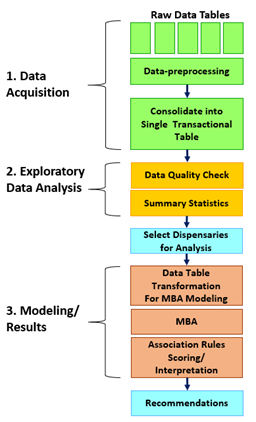
\includegraphics[width=0.8\linewidth]{figures/figure-1.png}
\captionof{figure}{Analytical approach used in this project.}
\label{fig:1}

\pdfbookmark[2]{Data Acquisition and Preprocessing}{Data Acquisition and Preprocessing}
\subsection{Data Acquisition and Preprocessing}

This project used an STS data set provided by the Washington State Liquor and Cannabis Board. Washington State uses a proprietary STS application from Leaf Data Systems \citep{leafdatasystems} which has collected data since 2018. The entire dataset consisted of 22 files ranging from 192 bytes to 5.5 GB in size. The combined dataset was over 29.8 GB. The size of the dataset made it too large to be explored and analyzed in its entirety on a conventional laptop, therefore I decided to use Google Cloud, a suite of cloud computing services, to carry out data storage, exploratory data analysis and modeling. I chose the R statistical programming language in a Jupyter Notebooks development environment for my exploratory data analysis and data modeling since it was also available as a service in the Google Cloud suite.

\par
The Google Cloud suite required a specific data encoding format for data imports called Unicode Transformation Format 8 (UTF-8) which is considered a standard for encoding tabular text data. The STS dataset posed a challenge in that it was encoded using UTF-16, a less common alternative to UTF-8, and a format incompatible with Google Cloud services. Additionally, the dataset was in tab delimited file format. This is not typically an issue for data imports into Google Cloud, but the decision was made to convert the dataset into the more common comma delimited file type as preventative measure to future issues.

\par
Carrying out the data encoding and file type translation presented a ``chicken and egg'' dilemma. Converting data encoding and file types is typically carried out by opening conventionally sized local files in a tool like Microsoft Excel and then saving them in the required format. This approach was not possible due to the size of most of the dataset files. Instead Microsoft PowerShell was used which is a Windows administrative scripting utility available on most Microsoft laptops. Using PowerShell allowed me to convert the files from their original format to UTF-8 comma delimited files without opening them. The large files took up to 6 hours to process. PowerShell scripting examples are available in Appendix A. Once properly converted all files were uploaded into the Google Cloud Storage service.

\par
Along with the STS data files, Washington State Liquor and Cannabis Board also supplied a data design document defining the various tables, fields, primary/secondary keys (table joins) used by the LEAF application. Based on the document, the following data schema was composed to complete the view of dispensary sales transactions (see \autoref{fig:2}). A complete singular transactional view of the data was prerequisite for MBA processing.

%\end{multicols*}
\begin{figure*}
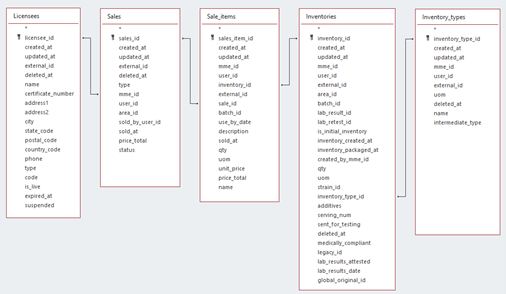
\includegraphics[width=0.8\linewidth]{figures/figure-2.png}
\captionsetup{margin=.1\linewidth}
\caption{A view of the five Seed to Sale retail data used in this analysis. Tables were joined by primary and secondary keys.}
\label{fig:2}
\end{figure*}
%\begin{multicols*}{2}

To give further context to the data here are short descriptions for each table in \autoref{fig:2} and how they are related:
\begin{itemize}
\item \texttt{Licensees} – This table is a listing of licensed facilities: producers, processors, testing labs, dispensaries, and transporters). Each licensee holds an official registration number issued by Washington State Liquor and Cannabis Board. This project only references licensed dispensaries. The \texttt{Licensees} table is linked to the \texttt{Sales} table by a unique licensee ID.

\item \texttt{Sales} – The sales table contains all wholesale and retail transactions with one unique sales identifier assigned to each transaction. This project only references retail sales. The \texttt{Sales} table is linked to \texttt{Sales\_Items} table via a unique \texttt{Sales} ID.

\item \texttt{Sale\_Items} – Each sale can contain a collection of one or more sale items. Each sale item has a product name and a unique identifier assigned. All products are assigned to a unique inventory ``lot'' so each sale item can be traced back to the original producer. The \texttt{Sale\_Items} table is linked to Inventories table via a unique \texttt{Sales\_Item} ID.

\item \texttt{Inventories} – Inventories are ``lots'' of products originating from growers and valued added processors. The \texttt{Inventories} table is linked to \texttt{Inventory\_Types} table via a unique Inventories ID.

\item \texttt{Inventory\_Types} – There are many inventory types ranging from originating products like ``Harvest Materials'' which are typically various types of cannabis flowers/buds to ``End Products'' like edibles, usable marijuana and concentrates for inhalation. This project only refers to end products sold through dispensaries. This table also has a unique identifier for each inventory type.
\end{itemize}

\pdfbookmark[2]{Data Quality and Exploratory Data Analysis}{Data Quality and Exploratory Data Analysis}
\subsection{Data Quality and Exploratory Data Analysis}

Data quality of STS source tables were verified once they were loaded into the Google Cloud Storage service \citep{MERINO2016123}. The Skimr reporting package for R (Using Skimr, 2021) was chosen to check table quality due to its convenience, coding simplicity and its comprehensive reports. A Skimr report was generated for each table which examined four variable types: character, logical, numeric and date. Reports were based on a 5\% simple random sample due to the number or records in each table. Skimr evaluated fields for missing values, completion rate, minimum value, maximum value, empty values, and unique values. Each report showed that the data quality was high with all required fields showing 100\% completion rates and all date fields falling within anticipated ranges (see Appendix B for an example of Skimr report results).

\par
Exploratory Data Analysis (EDA) queries were developed in Google BigQuery to gain a better business understanding of the five STS source tables' content. More specifically, exploratory queries were developed that identified which dispensaries made good candidates for MBA. To achieve this objective a query was written to join all five STS tables together into a single view of cannabis dispensary sales. Data was limited to the most recent calendar quarter available - 10/1/2020 to 12/31/2020. Since MBA's purpose is to identify useful product combinations in high volume transactional data when the product base is large \citep{agrawal1993mining} the main criteria for identifying the candidates were:
\begin{enumerate}
\item Dispensaries that had the highest transactional volume;
\item Dispensaries that had the greatest product mix;
\item Dispensaries that had the greatest earnings;
\item Dispensaries that represented three different socio-economic categories based on median household income (low, medium, high).
\end{enumerate}

The first three items above were used to generate an ordered list of candidates with the fourth point being used to select the three final top scoring dispensaries from their respective household median income categories. Washington state median household income data (by zip code) data was gathered from the US Census Bureau website \citep{medianincome}. The median income amounts were matched to each dispensaries' zip code. Once the candidate dispensaries were identified and matched to respective median household zip codes it was possible to move forward with the MBA process.

\pdfbookmark[2]{Dispensary Market Basket Analysis}{Dispensary Market Basket Analysis}
\subsection{Dispensary Market Basket Analysis}

This project's objective was to show if MBA can uncover purchasing patterns (association rules) in a large STS cannabis data set and to determine if those patterns were potentially useful for developing retail cross-selling strategies. The previous section outlined the process for consolidating the STS data into a usable set of sales transactions, but one additional data processing step was required as a prerequisite to using MBA that altered the structure of the transactional data from a ``tall'' table into a ``wide'' table.

\begin{figure*}
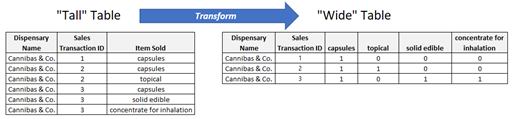
\includegraphics[width=0.8\linewidth]{figures/figure-3.png}
\captionsetup{margin=.1\linewidth}
\caption{Transforming a tall transactional table into a wide table.}
\label{fig:3}
\end{figure*}

% (Comprehensive R Archive Network (CRAN), 2021)

\par
\autoref{fig:3} illustrates the concept of transforming a tall table into a wide table. Transactional tables are sometimes called tall due the fact that retail PoS systems collect large numbers of sales records resulting in a long list of transactions. This project used the arules MBA algorithm in R \citep{arules} that required transaction data to be pivoted into a wide table where each product is given its own column as in \autoref{fig:3}.

\par
Every transaction shows a binary value for each product column depending on whether that product is present in the transaction. For example, in \autoref{fig:3} the tall table shows four possible products against transactions 1 through 3. Each one of the products is assigned its own column in the wide table with a 1 or a 0 being assigned if the product is present in a transaction. Transforming a long table in short table was done in R using the ``reshape'' function. A code example can be found in Appendix C. Once the data was pivoted into the correct form it was ready for MBA. 

\par
Running the arules MBA algorithm is relatively straightforward using only one line of R code but it requires two numeric input values: support and confidence. Selecting these two values was a subjective and iterative process based on the list of association rules generated. Recall from Chapter 2 that support is a measure of association rule ``popularity'' in relation to all the association rules generated form a data set. Also recall that confidence is the ``strength of association'' going from the left side of the rule (antecedent) to the right side of an association rule (consequent). Support was used as a filter to narrow rule set to the most significant items and confidence was adjusted to tease out those rules that had the highest level of association.

\par
By varying support and confidence values for each of the three dispensaries, several different visualizations were generated that expressed the relationships of the association rules. Greater context and intuition of the cannabis product rule space was gained. A graph matrix was used which shows how the various elements in the list of association rules are related. A scatter plot was used to show the relationship between support, confidence, and lift. Recall from chapter 2 that lift works the same way confidence does except it controls for how popular the consequent is. Lift values greater than 1 show strength of association with larger values indicating more strength. After taking support and lift into consideration as the main measures a final list of association rules for all three dispensaries was developed. The final list was used as a source for cross-selling recommendations.

\pdfbookmark[1]{Results and Discussion}{Results and Discussion}
\section{Results and Discussion}
\label{sec:results-and-discussion}

The objective of this project was to analyze cannabis retails sales data to validate if product cross-selling suggestions can be generated through MBA association rules. The approach used to answer this question consisted of three steps: data acquisition, exploratory data analysis and modeling results. The specific activities around data acquisition was covered previously. Here we will outline which candidate dispensaries were selected for MBA analysis and the associations rules generated by MBA.

\begin{figure*}
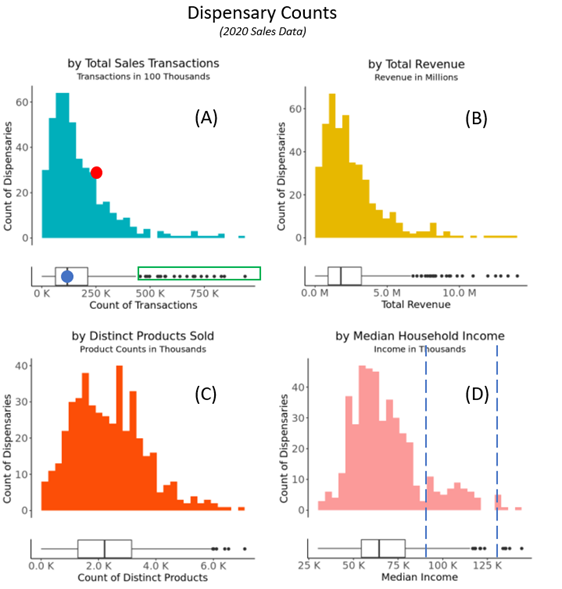
\includegraphics[width=0.8\linewidth]{figures/figure-4.png}
\captionsetup{margin=.1\linewidth}
\caption{The four charts depict the criteria that was used to select representative dispensaries for MBA.}
\label{fig:4}
\end{figure*}

\pdfbookmark[2]{Identifying Candidate Dispensaries for Market Basket Analysis}{Identifying Candidate Dispensaries for Market Basket Analysis}
\subsection{Identifying Candidate Dispensaries for Market Basket Analysis}

Before MBA modeling could be used to develop cross-selling association rules it was important to identify a list of representative dispensaries for analysis. As mentioned in chapter 3, four specific criteria were used to identify a list of candidate dispensaries for MBA. Those criteria were dispensaries with 1) the highest transactional volume, 2) the greatest product mix, 3) the highest earnings and 4) representation from low, medium, and high median regions. The first three criteria identified the most commercially active dispensaries with a diverse product set. The fourth criteria, median household income, was then applied to the top dispensaries to segment the market into three income demographics. The four criteria were applied to 2020 dispensary sales data.

\par
\autoref{fig:4} contains four histograms and boxplots combinations labeled A though D representing each of the previously mentioned four criteria. Each chart's histogram shows the relationship between the number dispensaries that fall within a criterion's range.

\par
For example, interpreting the red dot in \autoref{fig:4} (A) shows about 29 dispensaries had 250 thousand transactions for 2020. Additionally, the blue dot in the boxplot shows a mean transaction value of 125 thousand. The dispensaries of interest are the outliers to the right (green box). In this case these dispensaries offer the greatest transactional volume. Charts B and C work the same way but for total revenue and distinct products sold. Chart D shows how the count of dispensaries broke down by median household income. The two dashed lines indicate naturally occurring separation in income levels. I selected 0--85K, 85--125K and anything above 125K as my income buckets and labeled them low, medium, and high respectively. Once I had identified all four criteria, I combined them into a single representation so I could identify my top cannabis dispensaries from each income level (\autoref{fig:5}).

\begin{figure*}
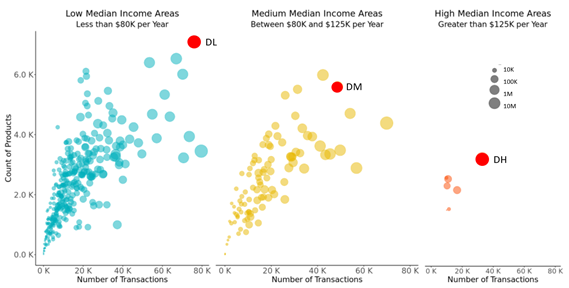
\includegraphics[width=0.8\linewidth]{figures/figure-5.png}
\captionsetup{margin=.1\linewidth}
\caption{Dispensary Comparison by Levels of Median Household Income.}
\label{fig:5}
\end{figure*}

\par
Each of the three charts above represent a level of median household income (low, medium, high). The remaining three dispensary selection criteria are represented in the charts like this:
\begin{enumerate}
\item Highest transactional volume = X-axis;
\item Greatest product mix = Y-axis;
\item Greatest earnings = Size of bubble .
\end{enumerate}

\par
The red dots in the upper right side of each chart identify the selected dispensary based on the highest criteria values. There were several dispensaries in the median income chart that could have been selected. The dispensary that made the best trade--off in criteria values was selected. \autoref{tab:1} lists the three dispensaries selected for the final MBA analysis.

\begin{table*}
  \setlength{\tabcolsep}{7pt}
  \sffamily \footnotesize \captionof{table}{Dispensary totals sales, transactions, and product counts.}
  \label{tab:1}
  \vspace{-.75\baselineskip}
  \colorbox{Gray}{%
    \begin{tabular*}{\linewidth}{
      C{1.25cm}
      C{2.15cm}
      C{3.05cm}
      R{1.25cm}
      R{2.15cm}
      R{1.9cm}
      R{1.75cm}
      R{1.25cm}
    }
      \toprule[0.5pt]
      \begin{tabular*}{1.25cm}{c}      
        Label
      \end{tabular*} &
      \begin{tabular*}{2.15cm}{c}
        Median \\ Income Level
      \end{tabular*} &
      \begin{tabular*}{3.05cm}{c}
        Dispensary Name
      \end{tabular*} &
      \begin{tabular*}{1.25cm}{c}
        ZIP Code
       \end{tabular*} &
      \begin{tabular*}{2.15cm}{c}
        Median Income \\ by ZIP
      \end{tabular*} &
      \begin{tabular*}{1.9cm}{c}
        Total Sales
      \end{tabular*} &
      \begin{tabular*}{1.75cm}{c}
        Total \\ Transactions
      \end{tabular*} &
      \begin{tabular*}{1.25cm}{c}
        Product \\ Count
      \end{tabular*} \\
      \midrule[0.5pt]
      DL & Low & Zips Cannabis & 98408 & \$59,207 & \$12,510,607 & 761,858 & 7,095 \\
      DM & Medium & PRC & 98223 & \$88,295 & \$7,357,044 & 486,777 & 5,598 \\
      DH & High & Green Theory Factoria & 98006 & \$144,247 & \$5,704,415 & 329164 & 3,212 \\
      \bottomrule[0.5pt]
    \end{tabular*}%
  }
\vspace{0.25\baselineskip}\\
% TODO: Add data source.
%{\scriptsize Data Source: \citeauthor{Facilities-Data}.}
\end{table*}

\pdfbookmark[2]{Market Basket Analysis Findings}{Market Basket Analysis Findings}
\subsection{Market Basket Analysis Findings}

MBA generates lists of product combinations from retail sales data. The resulting association rules are used promote cross-selling opportunities in complimentary products \citep{malati2017}. As mentioned in Chapter 2, this analysis used two primary measures to generate rules sets: support and confidence. Support can be thought of as a rule's popularity when compared with all other rules sets. Support values are measured in percentages and it is not uncommon for the values to be in the low single percentages when there are many products represented in a data set. Confidence was the second measure used to generate rule sets which can be thought of as the strength of the relationship between a rules first element and second element. Confidence values are also measured in percentages but are not typically as low as support percentages.

\par
Various combinations of support and confidence values were tried during the analysis of the three dispensary data sets. If the support and confidence values were set too low, then there was a chance of generating large ``noisy'' sets with low value rules. Balancing the two thresholds to generate a useful and reasonably sized rule set was the objective. \autoref{fig:6} shows a support vs. confidence scatter plot which incorporated a support value of 0.004 and a confidence value of 0.4 into the MBA algorithm.

\begin{center}
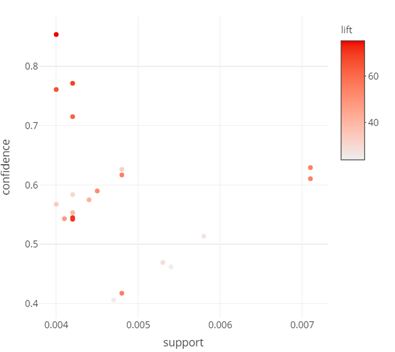
\includegraphics[width=0.8\linewidth]{figures/figure-6.png}
\end{center}
\captionof{figure}{Confidence vs. Support scatter plot.}
\label{fig:6}
\vspace{\baselineskip}

\par
Notice that the plot area is not inundated with data points. This means that the topmost data points are represented in terms of support, confidence, and lift. If any of the thresholds were lowered more data points would be present in the chart.

\par
The additional legend on the right side of \autoref{fig:6} represents lift. Lift is like confidence in that it indicates the likelihood of the combination, but the strength of association is bidirectional between the two elements whereas confidence is unidirectional. Lift was used as the key metric to identify ``close couplings'' for potential cross-selling opportunities. The stronger the bond between the rule elements the greater the lift value. Based on a support of 0.004 and a confidence of 0.4 the MBA algorithm produced 21 rule sets from the DL data as represented by the red dots in \autoref{fig:6}. The top ten resulting rules are listed in \autoref{tab:2} and follow an ``if-then'' format. For instance, the first DL rule:
\begin{equation*}
\begin{split}
\{\text{Wax} - \text{Chernobyl} - 01.0 g, \text{Wax} - \text{Pink} \#1 - 01.0 g\} \Rightarrow \\
\{\text{Wax} - \text{Starfighter} - 01.0 g\}
\end{split}
\end{equation*}

\noindent Reads like this:

\begin{quote}
{\itshape ``If Wax - Chernobyl - 01.0 g and Wax - Pink \#1 - 01.0 g are purchased together, then Wax - Starfighter - 01.0 g is also likely to be purchased''}
\end{quote}

\par
Additionally, the DM and DH dispensary top 10 rule sets can be seen in tables 3 and 4 respectively. All tables include the support and confidence values used to generate the rule sets.

\par
The final three tables confirm that MBA can generate product rules sets from STS cannabis dispensary data. There rules uncovered here are the basis for developing cross-selling opportunities for complimentary cannabis products.

\pdfbookmark[2]{Discussion}{Discussion}
\subsection{Discussion}

Analysis of the three dispensary MBA rule sets has confirmed MBA can be applied to retail cannabis data and has also uncovered some interesting observations. The DL association rules in \autoref{tab:2} show that wax products (wax products are infused with cannabis' main psychoactive chemical, THC, and are typically smoked or vaporized) were the only type of product represented in the top ten rules. Further analysis of all 21 rules show the same pattern of wax-only association rules suggesting that this dispensary may focus on wax product sales. The combinations of wax products in \autoref{tab:2} creates a potential opportunity for DL to cross-promote those combinations either through product placement, advertising, or salesperson recommendations.

\par
\autoref{tab:3}'s list of product combinations offers a different view of top ten product combinations. Like DL, DM shows rules that include wax products but in addition we see blunt combinations. A blunt is the common term for a hollowed-out cigar filled with cannabis. Interestingly blunts are only bought with other blunts and the same holds for the waxes indicating that these products may not be complimentary from the consumers perspective. Analysis shows 24 of the 34 DM rules show a consistent pattern of wax-to-wax or blunt-to-blunt combinations.

\begin{table*}
  \setlength{\tabcolsep}{6pt}
  \sffamily \footnotesize \captionof{table}{Top 10 Association Rules for low median income dispensaries.}
  \label{tab:2}
  \vspace{-.75\baselineskip}
  \colorbox{Gray}{%
    \begin{tabular*}{\linewidth}{
      L{12cm}
      C{1.6cm}
      C{2.05cm}
      C{1cm}
    }
      \toprule[0.5pt]
      \begin{tabular*}{12cm}{c}      
        Top 10 DL Association Rules
      \end{tabular*} &
      \begin{tabular*}{1.6cm}{c}
        Support
      \end{tabular*} &
      \begin{tabular*}{2.05cm}{c}
        Confidence
      \end{tabular*} &
      \begin{tabular*}{1cm}{c}
        ~Lift
       \end{tabular*} \\
      \midrule[0.5pt]
      \{Wax - Chernobyl - 01.0 g, Wax - Pink \# 1 - 01.0 g\} $\Rightarrow$ \{Wax - Starfighter - 01.0 g\} & 0.0040 & 0.8537 & 75.3223 \\
      \{Wax - Lemon OG - 01.0 g\} $\Rightarrow$ \{Wax - Pink Panther - 01.0 g\} & 0.0042 & 0.5423 & 70.3375 \\
      \{Wax - Pink Panther - 01.0 g\} $\Rightarrow$ \{Wax - Lemon OG - 01.0 g\} & 0.0042 & 0.5450 & 70.3375 \\
      \{Wax - God's Gift - 01.0 g, Wax - Chernobyl - 01.0 g\} $\Rightarrow$ \{Wax - Starfighter - 01.0 g\} & 0.0042 & 0.7714 & 68.0668 \\
      \{Wax - Pink \# 1 - 01.0 g, Wax - Starfighter - 01.0 g\} $\Rightarrow$ \{Wax - Chernobyl - 01.0 g\} & 0.0040 & 0.7609 & 65.1410 \\
      \{Wax - God's Gift - 01.0 g, Wax - Starfighter - 01.0 g\} $\Rightarrow$ \{Wax - Chernobyl - 01.0 g\} & 0.0042 & 0.7152 & 61.2338 \\
      \{Wax - Lemon OG - 01.0 g\} $\Rightarrow$ \{Wax - Blueberry Muffin - 01.0 g\} & 0.0048 & 0.6169 & 53.8835 \\
      \{Wax - Blueberry Muffin - 01.0 g\} $\Rightarrow$ \{Wax - Lemon OG - 01.0 g\} & 0.0048 & 0.4175 & 53.8835 \\
      \{Wax - Starfighter - 01.0 g\} $\Rightarrow$ \{Wax - Chernobyl - 01.0 g\} & 0.0071 & 0.6293 & 53.8727 \\
      \{Wax - Chernobyl - 01.0 g\} $\Rightarrow$ \{Wax - Starfighter - 01.0 g\} & 0.0071 & 0.6106 & 53.8727 \\
      \bottomrule[0.5pt]
    \end{tabular*}%
  }
\vspace{0.001\baselineskip}\\
\begin{tabular*}{\linewidth}{llll}
\multicolumn{4}{l}{\scriptsize Notes: Support = 0.004, Confidence = 0.40, and Total Rules Generated = 21.}
\end{tabular*}%
%\vspace{0.25\baselineskip}\\
% TODO: Add data source.
%{\scriptsize Data Source: \citeauthor{Facilities-Data}.}
\end{table*}

\begin{table*}
  \setlength{\tabcolsep}{6pt}
  \sffamily \footnotesize \captionof{table}{Top 10 Association Rules for medium median income dispensaries.}
  \label{tab:3}
  \vspace{-.75\baselineskip}
  \colorbox{Gray}{%
    \begin{tabular*}{\linewidth}{
      L{12cm}
      C{1.6cm}
      C{2.05cm}
      C{1cm}
    }
      \toprule[0.5pt]
      \begin{tabular*}{12cm}{c}      
        Top 10 DM Association Rules
      \end{tabular*} &
      \begin{tabular*}{1.6cm}{c}
        Support
      \end{tabular*} &
      \begin{tabular*}{2.05cm}{c}
        Confidence
      \end{tabular*} &
      \begin{tabular*}{1cm}{c}
        ~~Lift
       \end{tabular*} \\
      \midrule[0.5pt]
      \{\# Blunt Sativa\} $\Rightarrow$ \{\# Blunt Hybrid\} & 0.0012 & 0.4091 & 151.0130 \\
      \{\# Blunt Hybrid\} $\Rightarrow$ \{\# Blunt Sativa\} & 0.0012 & 0.4286 & 151.0130 \\
      \{\# Blunt Indica\} $\Rightarrow$ \{\# Blunt Hybrid\} & 0.0011 & 0.4359 & 160.9084 \\
      \{\# Blunt Hybrid\} $\Rightarrow$ \{\# Blunt Indica\} & 0.0011 & 0.4048 & 160.9084 \\
      \{Wax - Chocolate Trip - 01.0 g\} $\Rightarrow$ \{Wax - Timewreck - 01.0g\} & 0.0011 & 0.2464 & ~~~52.3264 \\
      \{Wax - Timewreck - 01.0 g\} $\Rightarrow$ \{Wax - Chocolate Trip - 01.0g\} & 0.0011 & 0.2329 & ~~~52.3264 \\
      \{Wax - Chocolate Trip - 01.0 g\} $\Rightarrow$ \{Wax - Ninja Nectar - 01.0g\} & 0.0011 & 0.2464 & ~~~32.3714 \\
      \{Wax - Ninja Nectar - 01.0 g\} $\Rightarrow$ \{Wax - Chocolate Trip - 01.0g\} & 0.0011 & 0.1441 & ~~~32.3714 \\
      \{Wax - American Pie - 01.0 g\} $\Rightarrow$ \{Wax - Lodi Dodi - 01.0g\} & 0.0013 & 0.2667 & ~~~29.9594 \\
      \{Wax - Lodi Dodi - 01.0 g\} $\Rightarrow$ \{Wax - American Pie - 01.0g\} & 0.0013 & 0.1449 & ~~~29.9594 \\
      \bottomrule[0.5pt]
    \end{tabular*}%
  }
\vspace{0.001\baselineskip}\\
\begin{tabular*}{\linewidth}{llll}
\multicolumn{4}{l}{\scriptsize Notes: Support = 0.001, Confidence = 0.01, and Total Rules Generated = 34.}
\end{tabular*}%
%\vspace{0.25\baselineskip}\\
% TODO: Add data source.
%{\scriptsize Data Source: \citeauthor{Facilities-Data}.}
\end{table*}

\begin{table*}
  \setlength{\tabcolsep}{6pt}
  \sffamily \footnotesize \captionof{table}{Top 10 Association Rules for low median income dispensaries.}
  \label{tab:4}
  \vspace{-.75\baselineskip}
  \colorbox{Gray}{%
    \begin{tabular*}{\linewidth}{
      L{12cm}
      C{1.6cm}
      C{2.05cm}
      C{1cm}
    }
      \toprule[0.5pt]
      \begin{tabular*}{12cm}{c}      
        Top 10 DM Association Rules
      \end{tabular*} &
      \begin{tabular*}{1.6cm}{c}
        Support
      \end{tabular*} &
      \begin{tabular*}{2.05cm}{c}
        Confidence
      \end{tabular*} &
      \begin{tabular*}{1cm}{c}
        ~Lift
       \end{tabular*} \\
      \midrule[0.5pt]
      \{Legend of Nigeria Prerolls 1g\} $\Rightarrow$ \{Jack Herer Prerolls 1g\} & 0.0011 & 0.2407 & 46.3627 \\
      \{Jack Herer Prerolls 1g\} $\Rightarrow$ \{Legend of Nigeria Prerolls 1g\} & 0.0011 & 0.2167 & 46.3627 \\
      \{Panda Fruit Drops- Green Apple 100mg\} $\Rightarrow$ \{Panda Fruit Drops- Peach Mango 100mg\} & 0.0010 & 0.2791 & 44.1733 \\
      \{Panda Fruit Drops- Peach Mango 100mg\} $\Rightarrow$ \{Panda Fruit Drops- Green Apple 100mg\} & 0.0010 & 0.1644 & 44.1733 \\
      \{Panda Fruit Drops- Strawberry Kiwi 100mg\} $\Rightarrow$ \{Panda Fruit Drops- Peach Mango 100mg\} & 0.0012 & 0.2500 & 39.5719 \\
      \{Panda Fruit Drops- Peach Mango 100mg\} $\Rightarrow$ \{Panda Fruit Drops- Strawberry Kiwi 100mg\} & 0.0012 & 0.1918 & 39.5719 \\
      \{Blueberry Belts - 100mg\} $\Rightarrow$ \{Apple Rings - 100mg\} & 0.0015 & 0.2787 & 38.7981 \\
      \{Apple Rings - 100mg\} $\Rightarrow$ \{Blueberry Belts - 100mg\} & 0.0015 & 0.2048 & 38.7981 \\
      \{Lodi Dodi .5g Preroll 2 pk\} $\Rightarrow$ \{Narnia .5g Preroll 2 pk\} & 0.0016 & 0.2727 & 37.0749 \\
      \{Narnia .5g Preroll 2 pk\} $\Rightarrow$ \{Lodi Dodi .5g Preroll 2 pk\} & 0.0016 & 0.2118 & 37.0749 \\
      \bottomrule[0.5pt]
    \end{tabular*}%
  }
\vspace{0.001\baselineskip}\\
\begin{tabular*}{\linewidth}{llll}
\multicolumn{4}{l}{\scriptsize Notes: Support = 0.001, Confidence = 0.01, and Total Rules Generated = 48.}
\end{tabular*}%
%\vspace{0.25\baselineskip}\\
% TODO: Add data source.
%{\scriptsize Data Source: \citeauthor{Facilities-Data}.}
\end{table*}

\par
\autoref{tab:4}'s DH rule set represents the highest mean income demographic of all three groups and shows a departure from the products listed in the DL and DM rule sets. Here we see no wax products at all and instead we see prerolls (a pre-rolled cannabis cigarette) and edibles (referred to as drops, rings, and belts in the rule sets). Again, these two classes of products are bought independently of each other. Analysis of the remaining 48 rules also list extracts for inhalation in the rule set, but again, these products appear to be bought in combination with the same product types. Although we see various of cross-selling opportunities in all three rules sets this initial analysis appears to show a ``barrier'' to mixing product categories which is not typically present in MBA. Traditional retail MBA, especially in grocery store sales, show a mix of products, as we would expect. Dispensaries seem to show that consumers are connoisseurs of specific products with little propensity to mix and match outside their area of preference. Would this self-selecting behavior limit the applicability to cross-selling between main product categories? Conducting an analysis of a larger sample of dispensaries would need to be carried out to confirm if this product cross-selling barrier truly exists.

\pdfbookmark[2]{Limitations and Recommendations}{Limitations and Recommendations}
\subsection{Limitations and Recommendations}

As previously explained, MBA rules for cross-selling opportunities are generated using support and confidence thresholds. Although these values are relative, low thresholds indicate that there are many low value rule combinations. Ideally rules with higher support, confidence values have more utility. In this analysis all three sets of rules had small support and confidence values. This can be result of a few factors. High product churn can introduce and take away product combinations injecting low value noisy combinations into market before they have a chance to mature and rise to the top. Complex product naming schemes, like we see in the cannabis data set, can also introduce a high level of granularity whereas assigning products to representative categories can strengthen the probability of generating stronger rule sets. Two possible next steps emerge from these observations. First, conducting a product churn analysis would uncover to what extent cannabis products are transient in the marketplace. Churn rules could be developed to filter the cannabis data set to make it more representative of strong product signals. Secondly, developing a cannabis product taxonomy would generate MBA rule sets into more meaningful product buckets. This would also help confirm if the product cross-selling barrier mentioned in the previous section truly exists. Additionally, a more meaningful product taxonomy would help confirm if segmentation by income impacts product purchasing combinations.

\pdfbookmark[1]{Conclusion}{Conclusion}
\section{Conclusion}
\label{sec:conclusion}

We have shown that market basket analysis (MBA) can be applied to a cannabis seed to sale (STS) dataset for the purpose of generating association rules. Furthermore, we have given examples how the resulting association rules can be used by three different cannabis dispensaries to generate cross-sell opportunities. This project has also uncovered observations that suggest there are further steps available to improve the effectiveness of MBA in this space. Based on the results of this study it is feasible for cannabis dispensaries or analytical service providers to conduct MBA analysis and potentially drive higher retail revenue in the cannabis market.

\par
Several key opportunities for follow on work emerged during this project. First, when conducting MBA on retail cannabis data is the size of the dataset itself. This project used data supplied by the Washington State Liquor and Cannabis Board. Some of the files provided were over 15 GB in size which necessitated the use of cloud services to ingest and preprocess the data before any meaningful analysis could be conducted. Those intent on working with large cannabis data sets in the future should consider encouraging state authorities to release their data through cloud services for easier public access.

\par
Another opportunity for future work regards how retail cannabis products are labeled before a meaningful MBA is attempted. MBA data relies on products that are labeled in such a way as to be reasonably descriptive. Multiple uniquely names products within a category may lower the quality of MBA results by injecting large numbers of meaningless combinations which was a limitation in this dataset. In a grocery store setting, labeling cleaning products as launder detergent and stain removers may yield better MBA rules sets than labeling all the various laundry detergents and stain removers with the brand name. Results from this project showed that overly granular labeling can potentially washout strong association rules necessary to identify cross-selling opportunities. Future work should consider the appropriate level of product labeling before the MBA analysis is conducted. This could take the form of developing a product taxonomy of labels for various cannabis product categories. The resulting taxonomy could then be applied to classifying each product accordingly creating stronger association rules signals.

\par
Additionally, effective MBA analysis requires that a stable list of products is offered over a reasonable period. Quickly introducing new products while rapidly taking away existing ones introduces product churn which prohibits strong association rules from maturing. It may be quite reasonable to expect new retail markets, like recreational cannabis, to initially see product churn. If that is the case, then alternatives to MBA should be considered to develop cross-selling opportunities. The limitations potentially imposed by project churn was not confirmed in this study but follow on work should consider developing churn models to detect and mitigate its presence in retail cannabis data sets.

\par
Finally, this project identified that customers do not typically mix and match product purchases outside of a main product family. If this affinity can be further confirmed, then It would be a great help to others conducting MBA in this space in showing that cross-selling opportunities may be more effectively executed if they are limited to specific product groupings.

%---------------------------------%
% References
%---------------------------------%
\nocite{*}
\pdfbookmark[1]{References}{References}
\bibliography{references}

%---------------------------------%
% End of the Body
%---------------------------------%
\end{multicols*}
\thispagestyle{regular}
\end{document}
